\documentclass[border=9,tikz]{standalone}
\begin{document}
\def\GroundBreaking{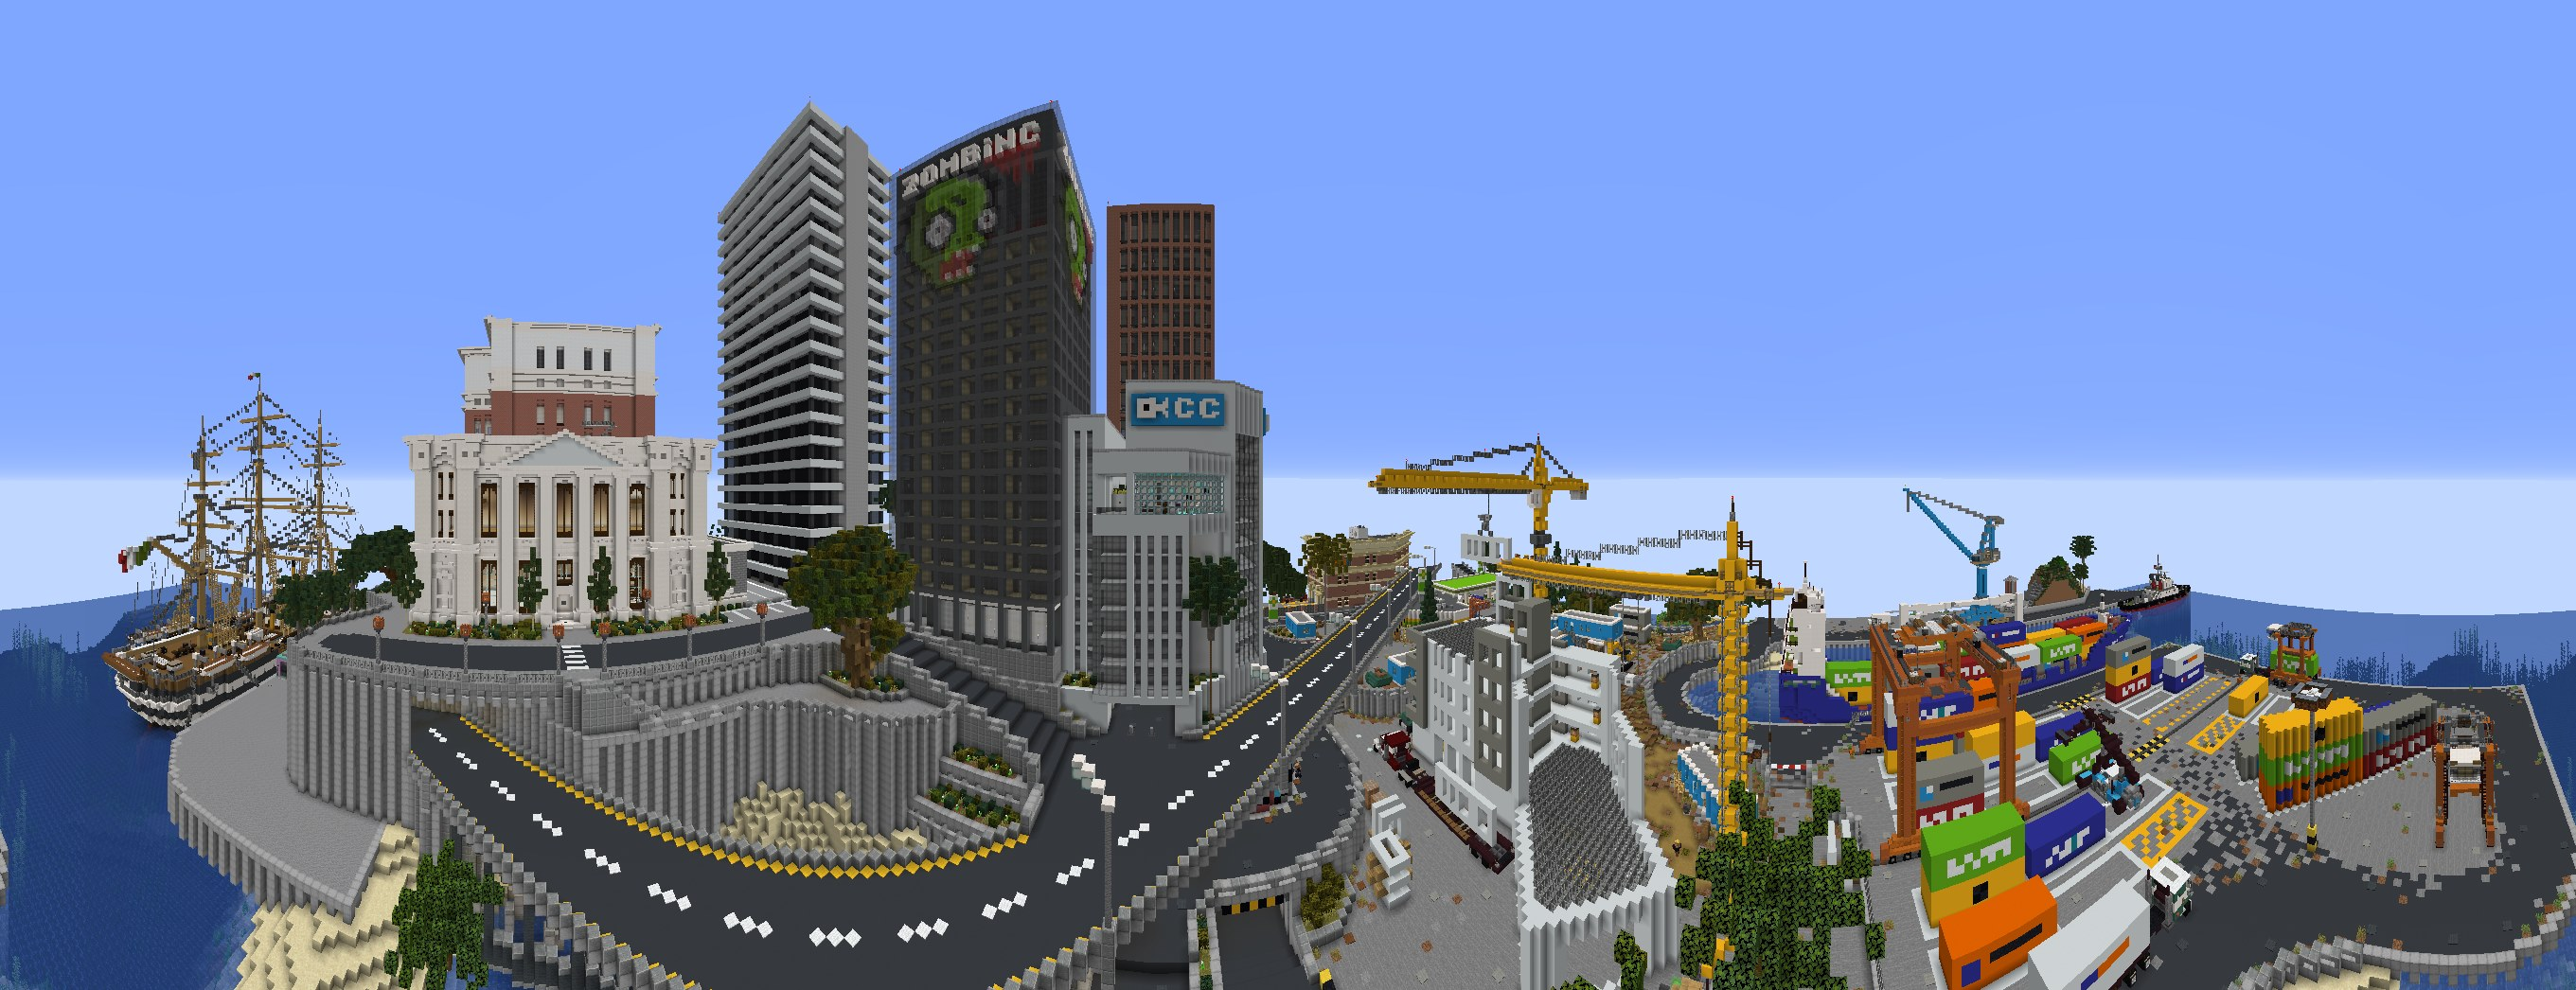
\includegraphics[width=6cm]{minecraft.jpg}\llap\LaTeX}
\def\RememberInversion(#1,#2){
	\expandafter\xdef\csname Inv(\u,\v)x\endcsname{\xx}
	\expandafter\xdef\csname Inv(\u,\v)y\endcsname{\yy}
}
\def\RecallInversion#1(#2,#3){
	\expandafter\xdef\csname#1x\endcsname{\csname Inv(#2,#3)x\endcsname}
	\expandafter\xdef\csname#1y\endcsname{\csname Inv(#2,#3)y\endcsname}
}
\tikz{
	\draw (0,0)circle(10);
	\foreach\u in{-30,...,30}{
		\foreach\v in{-11,...,11}{
			% transformation of (u, v), unit mm
			\pgfmathsetmacro\uu{\u + 30}
			\pgfmathsetmacro\vv{\v - 2}
			\pgfmathsetmacro\tt{\uu * 6}
			\pgfmathsetmacro\rr{exp(4 - \vv/22 -\uu/60)}
			\pgfmathsetmacro\xx{\rr * cos(\tt)}
			\pgfmathsetmacro\yy{\rr * sin(\tt)}
			% Remember the coordinates
			\RememberInversion(\u,\v)
		}
	}
	\foreach\u in{-30,...,29}{
		\foreach\v in{-11,...,10}{
			% For every square, recall the coordinates of the four corners
			\pgfmathtruncatemacro\U{\u+1}
			\pgfmathtruncatemacro\V{\v+1}
			\RecallInversion NW(\u,\V)\RecallInversion NE(\U,\V)
			\RecallInversion SW(\u,\v)\RecallInversion SE(\U,\v)
			% The lower left triangle ◺
			\pgfmathsetmacro\aa{\SEx-\SWx}\pgfmathsetmacro\ab{\SEy-\SWy}
			\pgfmathsetmacro\ba{\NWx-\SWx}\pgfmathsetmacro\bb{\NWy-\SWy}
			\pgflowlevelobj{
				\pgfsettransformentries\aa\ab\ba\bb{\SWx mm}{\SWy mm}
			}{
				\clip(1mm,0)-|(0,1mm)--cycle;
				\path(-\u mm,-\v mm)node{\GroundBreaking};
			}
			% The upper right triangle ◹
			\pgfmathsetmacro\aa{\NEx-\NWx}\pgfmathsetmacro\ab{\NEy-\NWy}
			\pgfmathsetmacro\ba{\NEx-\SEx}\pgfmathsetmacro\bb{\NEy-\SEy}
			\pgflowlevelobj{
				\pgfsettransformentries\aa\ab\ba\bb{\NEx mm}{\NEy mm}
			}{
				\clip(-1mm,0mm)-|(0mm,-1mm)--cycle;
				\path(-\U mm,-\V mm)node{\GroundBreaking};
			}
		}
	}
}

\end{document}